%%%%%%%%%%%%%%%%%%%%%%%%%%%%%%%%%%%%%%%%
% datoteka diploma.tex
%
% vzorčna datoteka za pisanje diplomskega dela v formatu LaTeX
% na UL Fakulteti za matematiko in fiziko
%
% vkup spravil Gašper Fijavž, december 2010 množica popravkov v januarju,
% februarju marcu 2011 verzijo 29. marec 2011 za FMF 19.9.2013 prilagodil Rok
% Mihevc
%%%%%%%%%%%%%%%%%%%%%%%%%%%%%%%%%%%%%%%%

\documentclass[a4paper, oneside, 12pt]{book}

\usepackage[utf8]{inputenc}
\usepackage[slovene,english]{babel}    % naloži, med drugim,
\usepackage[pdftex]{graphicx}  % omogoča vlaganje slik
\usepackage{fancyhdr}          % poskrbi, na primer, za
\usepackage{amssymb}           % dodatni simboli
\usepackage{amsmath}           % eqref, npr.
\usepackage{verbatim}
\usepackage{float}
\usepackage{tikz}

\renewcommand{\baselinestretch}{1.3} % ustrezen razmik med vrsticami

%oznake strani

\renewcommand{\chaptermark}[1]%
{\markboth{\MakeUppercase{\thechapter.\ #1}}{}} \renewcommand{\sectionmark}[1]
{\markright{\MakeUppercase{\thesection.\ #1}}} \renewcommand{\headrulewidth}{0.5pt} \renewcommand{\footrulewidth}{0pt} 
\fancyhf{}
\fancyhead[LE,RO]{\sl \thepage} \fancyhead[LO]{\sl \rightmark} \fancyhead[RE]{\sl \leftmark}

\newcommand{\BibTeX}{{\sc Bib}\TeX}

\newcommand{\autfont}{\Large} \newcommand{\titfont}{\LARGE\bf}
\newcommand{\clearemptydoublepage}{\newpage{\pagestyle{empty}\cleardoublepage}}
\setcounter{tocdepth}{1}	      % globina kazala

% konstrukti
\newtheorem{izrek}{Izrek}[chapter] \newtheorem{trditev}{Trditev}[izrek]
\newenvironment{dokaz}{\emph{Dokaz.}\ }{\hspace{\fill}{$\Box$}}

\begin{document}
\selectlanguage{slovene}
\frontmatter
\setcounter{page}{1}
\renewcommand{\thepage}{}

\thispagestyle{empty}
\begin{center}
  {\large\sc Univerza v Ljubljani\\
    Fakulteta za Matematiko in Fiziko\\
    Oddelek za Fiziko\\
  Univerzitetni študij, naravoslovna smer}
  \vskip 10em
  {\autfont Rok Mihevc \par}
  {\titfont Kraške vrtače Dinarskega krasa \par}
  {\vskip 2em \textsc{DIPLOMSKO DELO}\par}
  \vfill
  \null
  {\large \textsc{Mentor}: prof.\ dr.  Rudolf Podgornik\par}
    %  {\large \textsc{Somentor}:  izr.\ prof.\ dr. \par}%
  {\vskip 2em \large Ljubljana, 2014 \par}
\end{center}

\clearemptydoublepage \clearemptydoublepage

\vspace*{1cm}
\begin{center} {\Large \textbf{\sc Izjava o avtorstvu diplomskega dela}} \end{center}

  \vspace{1cm} \noindent Spodaj podpisani Rok Mihevc, z vpisno številko
  \textbf{28030017}, sem avtor  diplomskega dela z naslovom:

  \vspace{0.5cm} \emph{Kraške vrtače Dinarskega krasa}

  \vspace{1.5cm} \noindent S svojim podpisom zagotavljam, da: \begin{itemize}
    \item sem diplomsko delo izdelal samostojno pod mentorstvom prof.\ dr.\
      \mbox{Rudolfa} \mbox{Podgornika}, %in somentorstvom izr.\ prof.\ dr.\,

    \item	so elektronska oblika diplomskega dela, naslov (slov., angl.), povzetek
      (slov., angl.) ter ključne besede (slov., angl.) identični s tiskano obliko
      diplomskega dela \end{itemize}

      \vspace{1cm} \noindent V Ljubljani, dne . februarja 2014 \hfill Podpis avtorja:

    % prazna stran
      \clearemptydoublepage

      \begin{comment}
    %%%%%%%%%%%%%%%%%%%%%%%%%%%%%%%%%%%%%%%%
    % zahvala
      \thispagestyle{empty}\mbox{}\vfill\null\it% Staršema za podporo. \rm\normalfont

    % prazna stran
      \clearemptydoublepage

    %%%%%%%%%%%%%%%%%%%%%%%%%%%%%%%%%%%%%%%%
    % posvetilo
      \thispagestyle{empty}\mbox{}{\vskip0.20\textheight}\mbox{}\hfill\begin{minipage}{0.55\textwidth}%
        Svoji dragi Alenčici. \normalfont\end{minipage}

    % prazna stran
        \clearemptydoublepage

    %%%%%%%%%%%%%%%%%%%%%%%%%%%%%%%%%%%%%%%%
    % ODREZANA NASLOVNICA ITD. DO KAZALA
        \end{comment}

  % kazalo
        \def\thepage{}% preprecimo tezave s stevilkami strani v kazalu
        \tableofcontents{}

  % prazna stran
        \clearemptydoublepage

    %%%%%%%%%%%%%%%%%%%%%%%%%%%%%%%%%%%%%%%%
    % povzetek 
        \addcontentsline{toc}{chapter}{Povzetek} 
        \chapter*{Povzetek}

        Z numeričnimi metodami obdelamo $60 km^2$ velik digitalni model reliefa Menišije ločljivosti $1m^2$ in identificiramo veliko število kraških vrtač. Iz oblik velikega števila vrtač izračunamo povprečno obliko vrtače in jo analitično opišemo z gaussovo funkcijo. Odkrite realne vrtače nato prilegamo na gaussovo funkcijo, ter pogledamo porazdelitev parametrov le-te na našem vzorcu.

        Zaradi geološke zgodovine področja Menišije in medsebojne podobnosti vrtač na tem območju, postavimo tezo da jih je oblikoval isti geomorfološki proces, ki vodi do iste stabilne oblike, ki so jo vrtače na tem območju že dosegle.
        S pomočjo podatkov pridobljenih v prvem delu naloge predlagamo časovno statičen nastavek, ki analitično opiše najdene vrtače. Postavimo tezo, da vrtače nastanejo z difuzijo in predlagamo dinamičen nastavek za obliko vrtače in difuzijsko konstanto, ki rešita difuzijsko enačbo.

        \clearemptydoublepage

    %%%%%%%%%%%%%%%%%%%%%%%%%%%%%%%%%%%%%%%%
    % abstract
        \selectlanguage{english} \addcontentsline{toc}{chapter}{Abstract}
        \chapter*{Abstract}
        Abstract

        \selectlanguage{slovene}
    % prazna stran
        \clearemptydoublepage

        \mainmatter
        \setcounter{page}{1}
        \pagestyle{fancy}

        \chapter{Uvod}
        \label{uvod}

        \begin{figure}[H]
          \begin{center}
            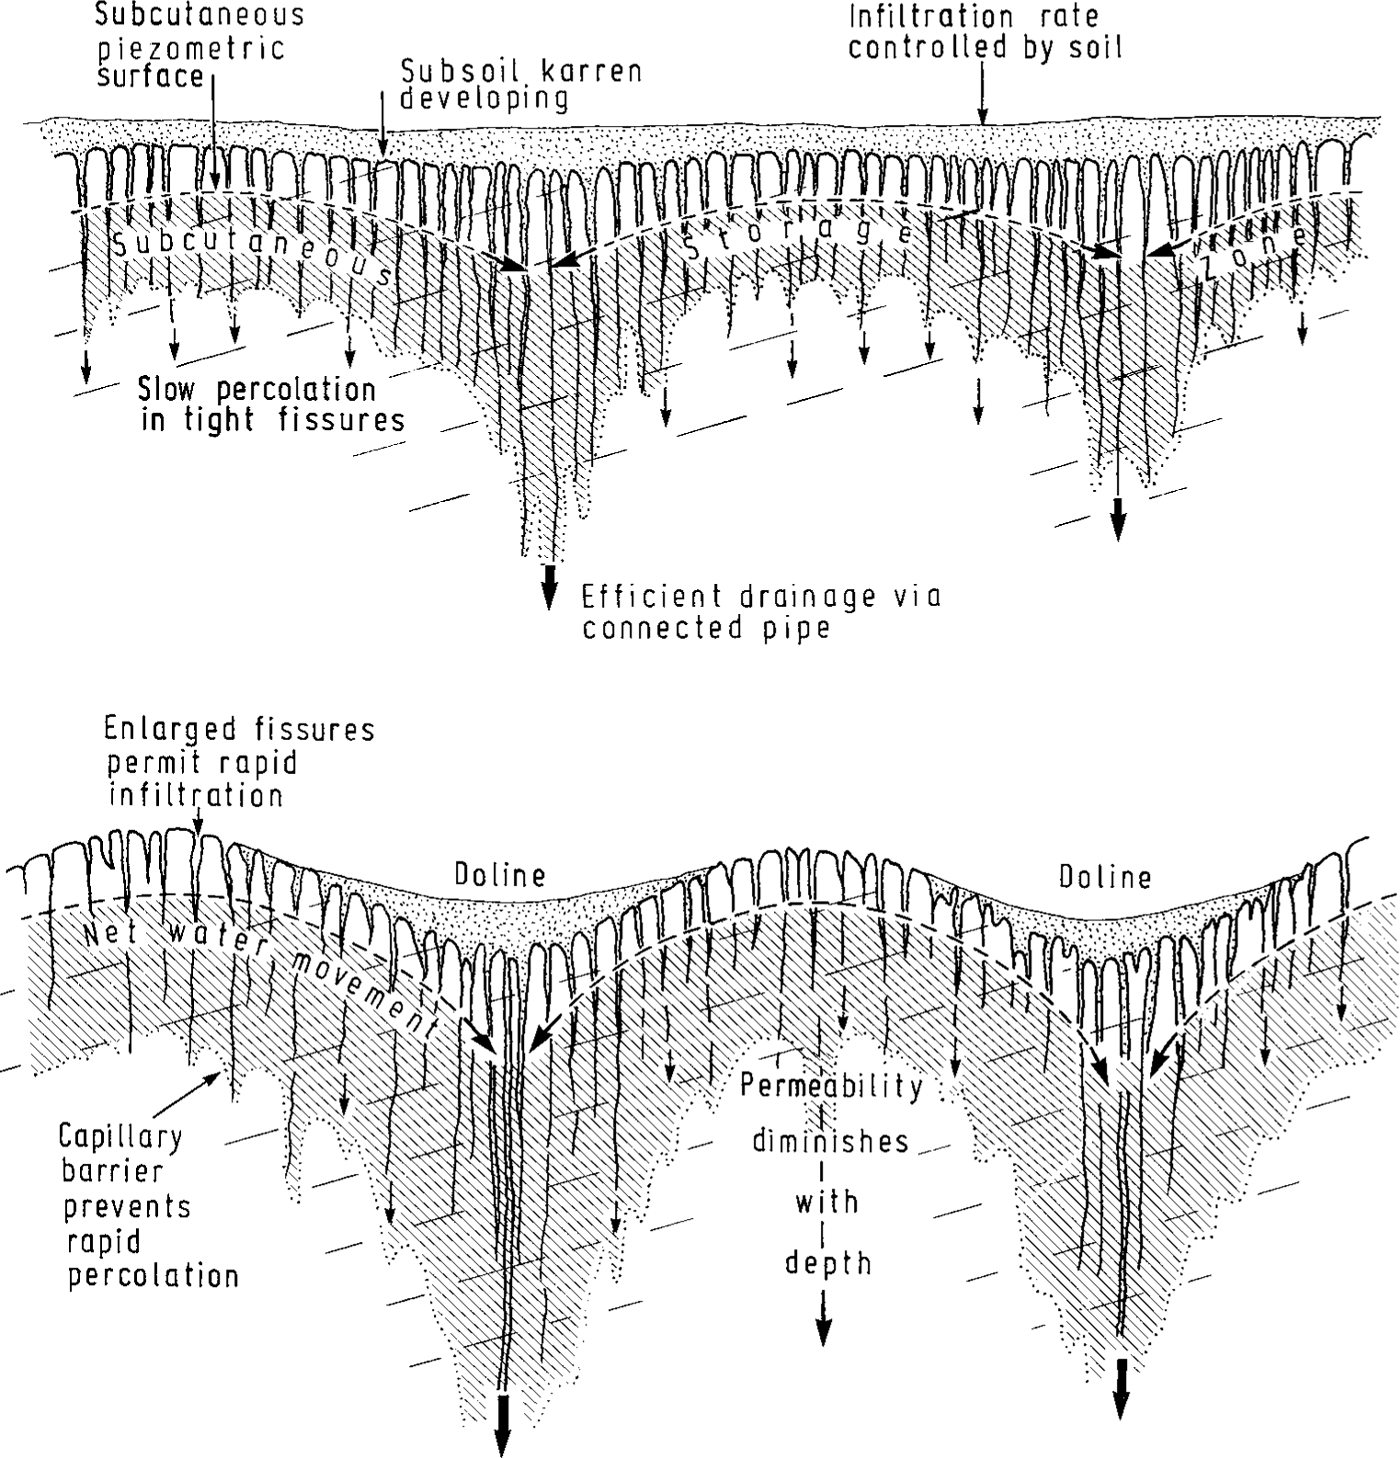
\includegraphics[width=10cm]{slike/vrtaca-ford-williams}
          \end{center}
          \caption{Priljubljena geomorfološka shema za razlago vrtač. Vir: \cite{ford2007karst}}
          \label{fig:vrtaca-ford-williams}
        \end{figure}

        Namen tega dela je na podlagi digitalnega modela reliefa dokumentirati in statistično preučiti velik vzorec realnih kraških vrtač na slovenskem Dinarskem krasu, predlagati analitično funkcijo, ki bi opisala idealno vrtačo, ter na podlagi le-te poiskusiti modelirati naravne procese, ki povzročajo nastanek in obliko vrtač.

        Vrtače so zaobljene lijakaste globeli, globine nekaj metrov in premera nekaj deset metrov. Obstaja več geomorfoloških modelov njihovega nastanka.

        Za študij realnih vrtač uporabimo digitalni model reliefa Menišije (Slika \ref{fig:menisija-karta}) ločljivosti 1m, ki omogoča zanesljivo identifikacijo in študij vrtač ter udornic (Slika \ref{fig:menisija-relief}).

        \begin{figure}[H]
          \centering
          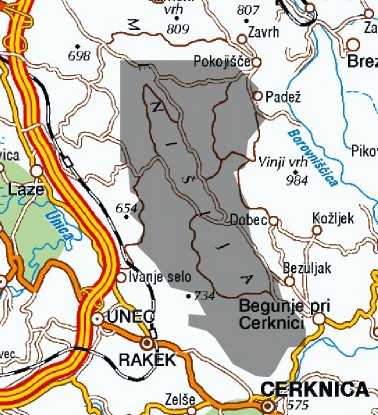
\includegraphics[width=8cm]{slike/menisija-karta}
          \caption{Menišija, $60 km^2$ veliko območje med Cerknico in Logatcem vsebuje nekaj tisoč vrtač in več udornic in predstavlja približno odstotek slovenskega krasa. Vir: Geopedia, Geodetski inštitut Slovenije}
          \label{fig:menisija-karta}
        \end{figure}

        Površje Menišije sestavljajo plasti krednega apnenca (starost nastanka 135-65 miljonov let), ki so na površje prišli zaradi dogodkov povezanih s podrivanjem Adriatske plošče (17-7 miljonov let). Menišija je bila uravnano kraško polje do 3.5 miljona let pred sedanjostjo, ko se je zaradi tektonske aktivnosti dvignila nad okolico in vzpostavljeni so bili hidrološki pogoji za nastanek vrtač. Hitrost zniževanja (denudacije) kraškega površja se ocenjuje na 20-50 m / miljon let, torej se je površje Menišije v času od nastanka znižalo za 70-175m, hkrati pa so se v njem pojavile vrtače, udornice in brezstrope jame. \cite{Vrabec2006} \cite{Placer2010}

        \begin{figure}[H]
          \begin{center}
            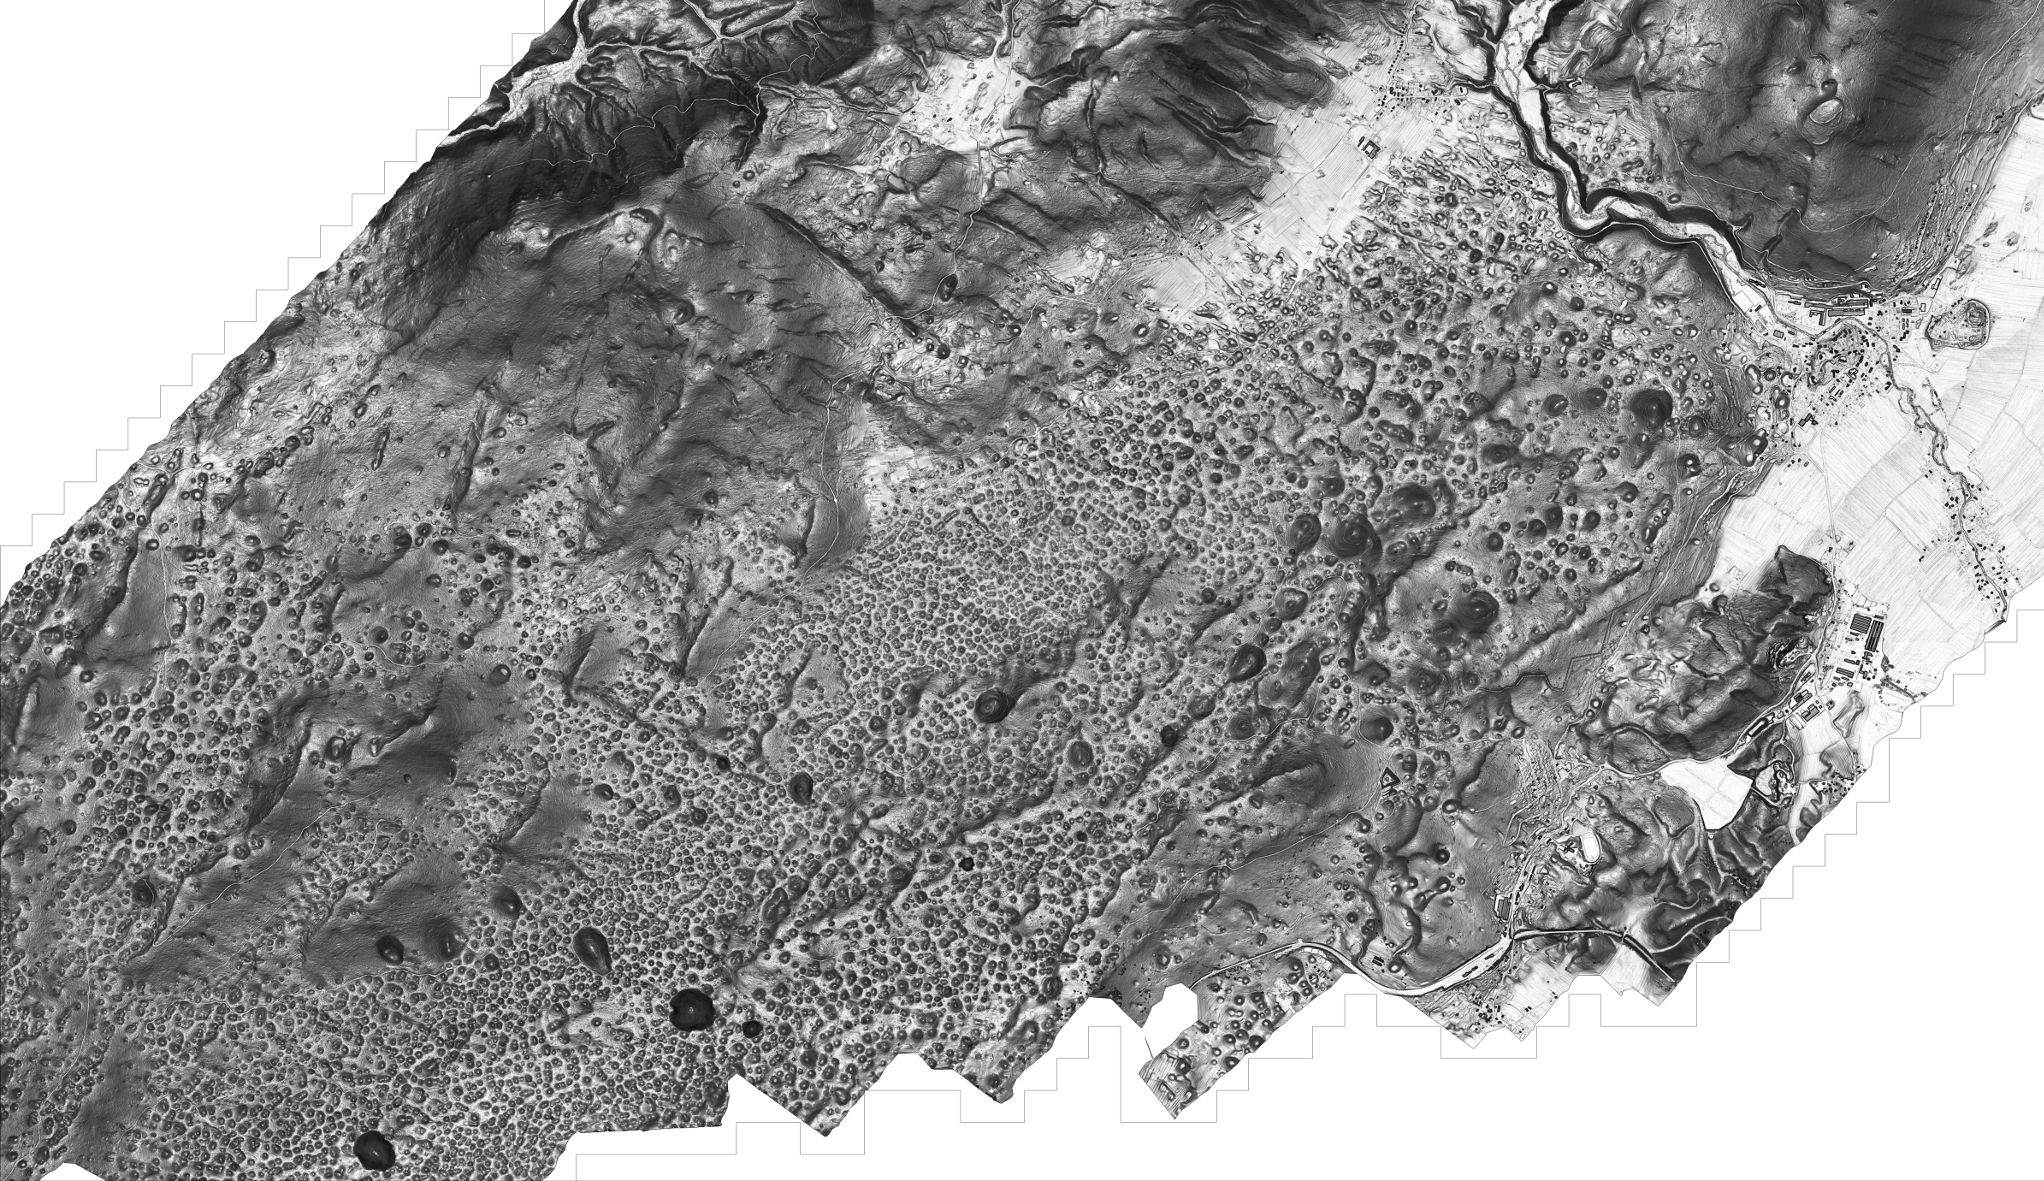
\includegraphics[width=12cm]{slike/menisija-relief}
          \end{center}
          \caption{Senčen 3D relief dela Menišije uporabljen v tej nalogi. Vir: Geodetski inštitur Slovenije \cite{LAK} po metodi \cite{Kobler20079}.}
          \label{fig:menisija-relief}
        \end{figure}
        \chapter{Preučevanje realnih vrtač}
        \label{realne-vrtace}
        Identifikacijo velike količine objektov se lotimo s segmentacijo po konkavnosti, kot predlaga \cite{doctor13}. Točke, ki so nižje od svoje okolice imajo nižji indeks konkavnosti, točke višje od svoje okolice pa višjega. Pri tem je pomembna tudi pametna izbiro okolice - od nje je odvisno kako velike konkavnosti bomo zaznali. Končno zavržemo konveksne dele površja in konkavne odberemo kot vrtače. Rezultat vidimo na sliki \ref{fig:menisija-vrtace}. Opaziti velja, da izbrana metoda segmetacije del robov konkavnih objektov klasificira kot konkavne in zato podceni radij. Za naše namene to ni pretirano moteče, saj to podcenitev zlahka kompenziramo kasneje.

        \begin{figure}[H]
          \begin{center}
            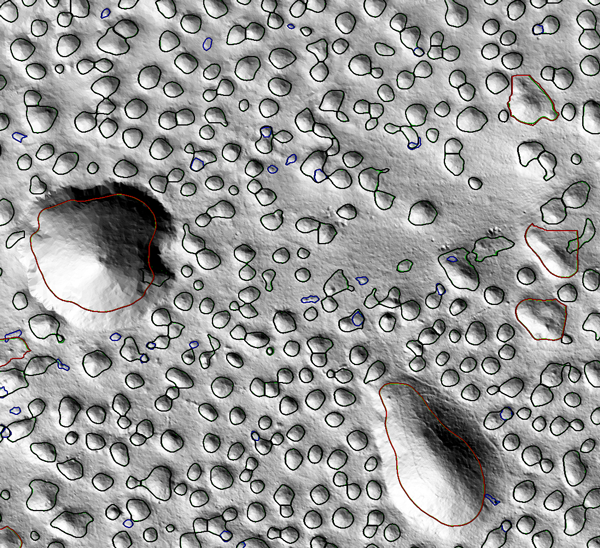
\includegraphics[width=13cm]{slike/menisija-vrtace}
          \end{center}
          \caption{Del od 8687 zaznanih konkavnih objektov na območju Menišije. Poleg vrtač so na sliki vidne tudi udornice.}
          \label{fig:menisija-vrtace}
        \end{figure}

        Najdeni konkavni objekti imajo porazdelitev efektivnih polmerov (\mbox{$r_{eff}=\sqrt{\frac{A_{eff}}{\pi}}$}), kot vidno na sliki \ref{fig:menisija-polmeri-hist}.

        \begin{figure}[H]
          \centering
          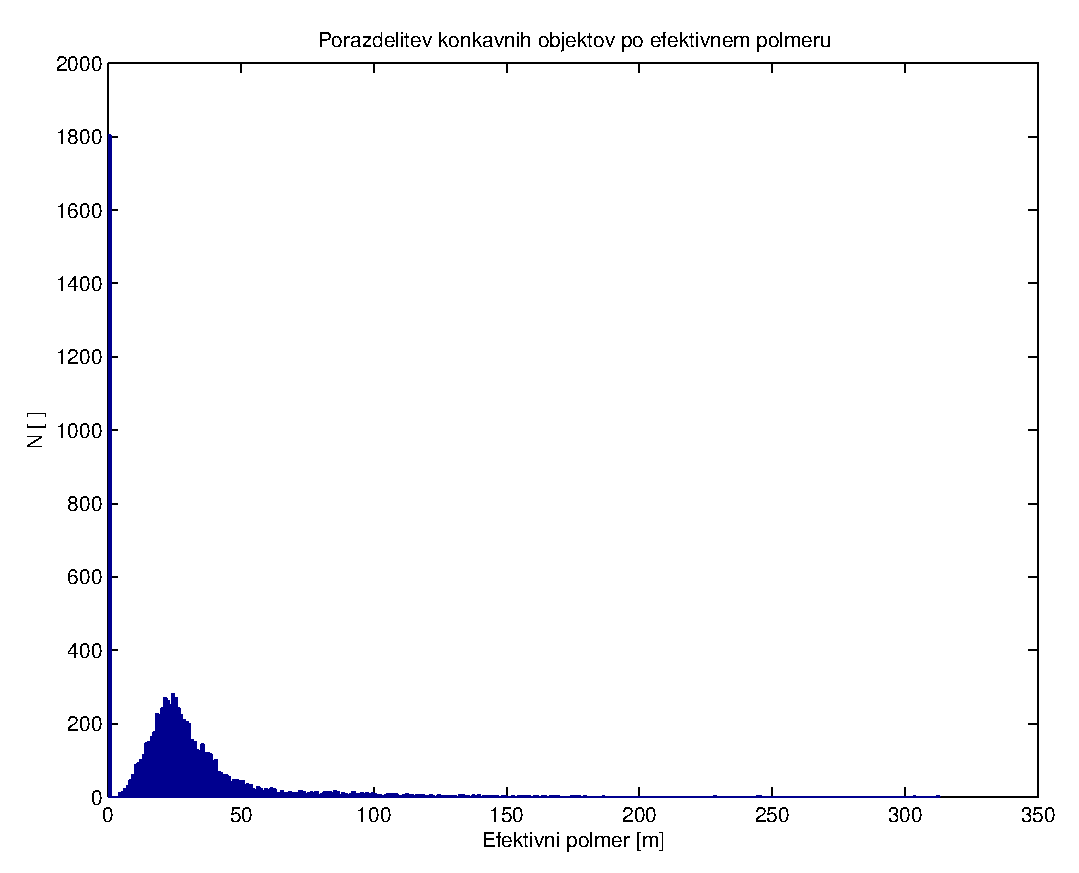
\includegraphics{slike/menisija-polmeri-hist}
          \caption{Polmeri konkavnih objektov v Menišiji, vrh pade v razred od 24m do 25m}
          \label{fig:menisija-polmeri-hist}
        \end{figure}

        To daje slutiti, da bodisi obstaja ravnovesna velikost vrtače, h kateri konvergirajo vse konkavne oblike v območju ne glede na njihov nastanek, bodisi da so vsi konkavni objekti v tem območju nastali v kratkem časovnem obdobju in se razvijali z enako hitrostjo. Odločimo se za raziskovanje prve možnosti.
        Predvidevamo torej, da obstaja ravnovesna oblika vrtače, ki bi se pojavila na idelani podlagi, če bi preteklo dovolj časa.

        Posamezne realne vrtače zaradi lokalnih pogojev in zgodovine razvoja reliefa niso simetrične, a zdi se, da so si med seboj podobne. Da bi ugotovili idealno obliko vrtače, izračunamo povprečje velikega števila realnih vrtač. Uporabimo dva pristopa - pri prvem (Slika \ref{fig:menisija-vrtaca}) vrtače različnih velikosti raztegnemo in povprečimo, pri drugem (Slika \ref{fig:menisija-vrtace-po-razredih}) pa jih razdelimo v velikostne razrede in jih povprečimo znotraj le-teh. 

        \begin{figure}[H]
          \centering
          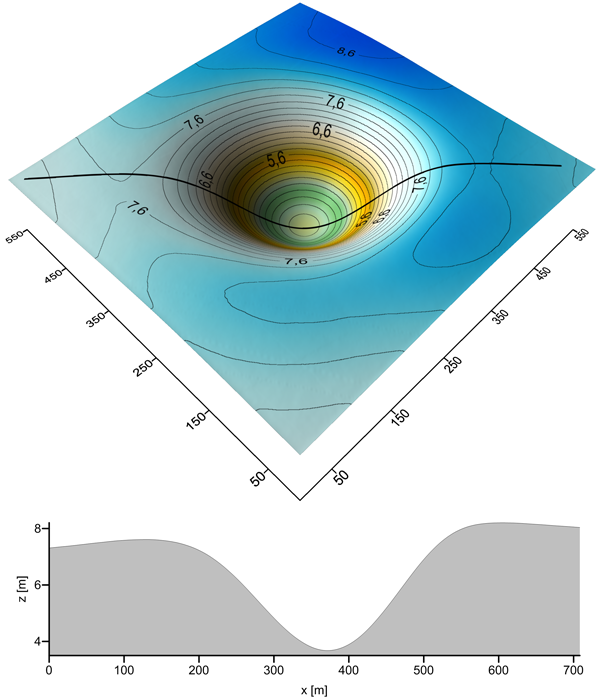
\includegraphics[width=13cm]{slike/menisija-vrtaca}
          \caption{Povprečje 8687 realnih vrtač z območja Menišije, pred povprečjem so bile vrtače raztegnjene na velikost največje v setu.}
          \label{fig:menisija-vrtaca}
        \end{figure}

        \begin{figure}
          \centering
          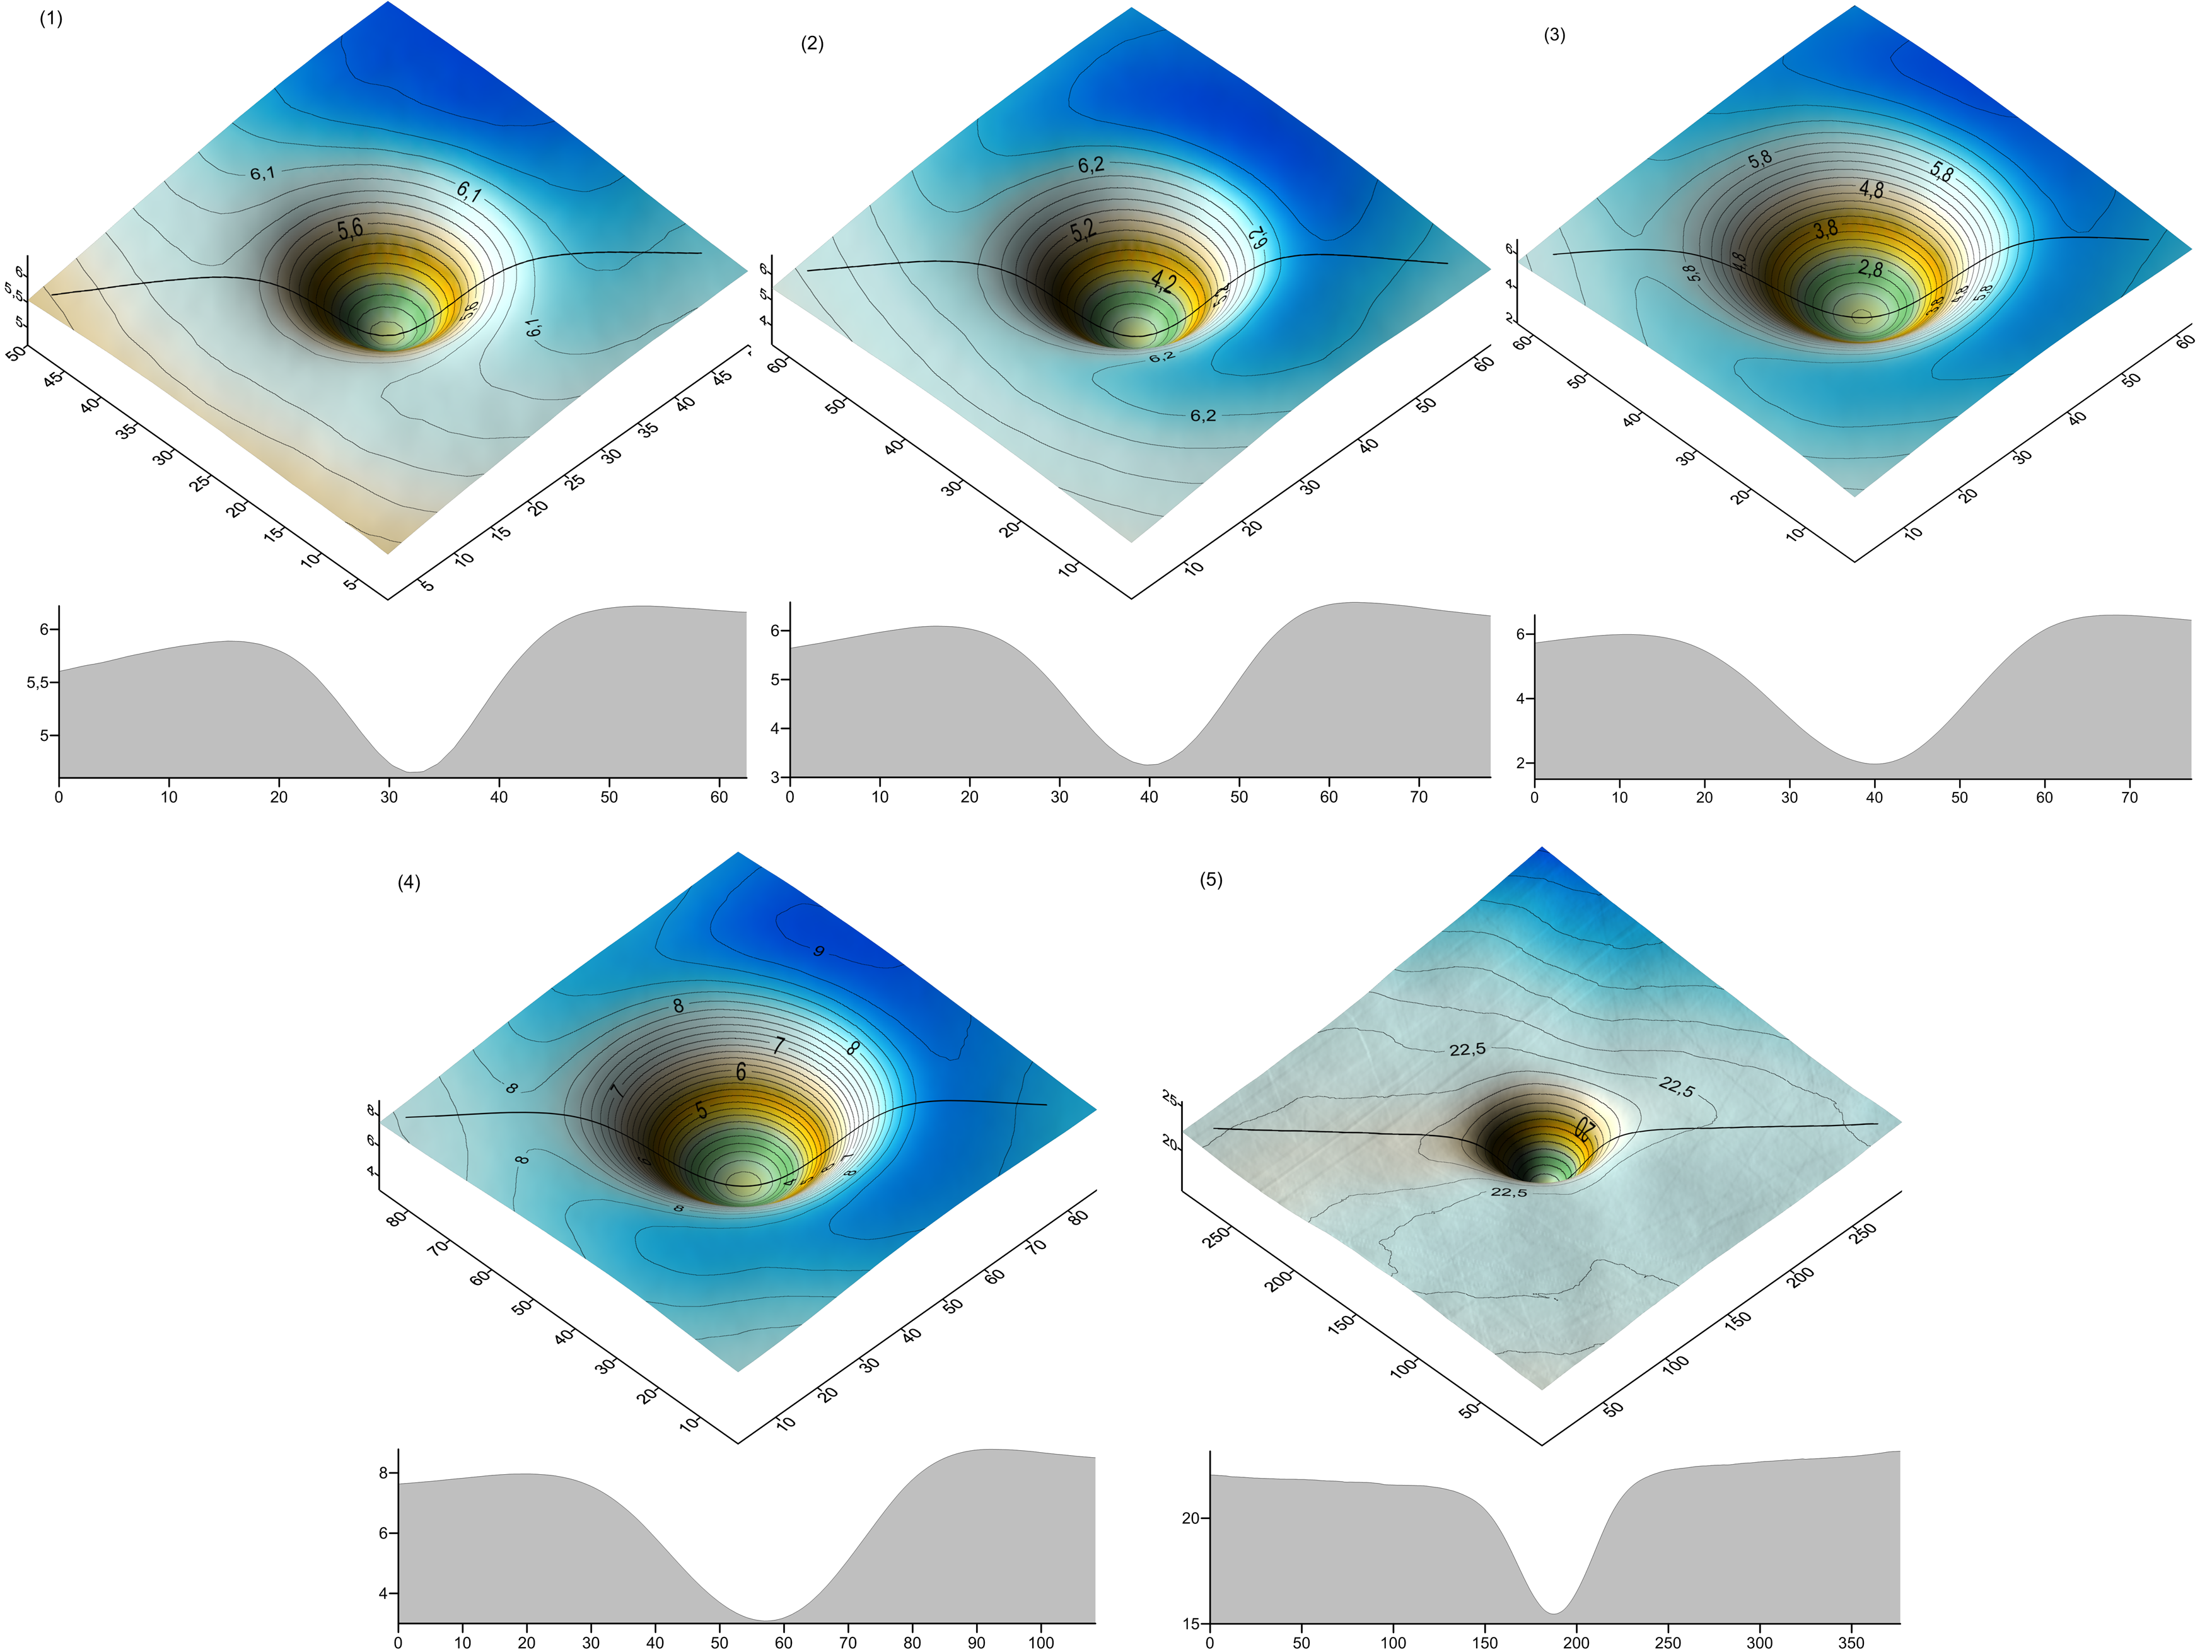
\includegraphics[width=19cm,angle=90]{slike/vrtace-po-razredih-menisija}
          \caption{Vrtače po velikosti razdelimo v pet razredov (najmanjša petina gre v prvi razred, itn.), in jih znotraj razredov povprečimo.}
          \label{fig:menisija-vrtace-po-razredih}
        \end{figure}

        Na prvi pogled se zdijo dobljeni profili gaussove oblike (\ref{fit-vrtace}), kar ne zbuja nujno zaupanja v metodo. Zdi pa se, da so oblike simetrične po kotu, torej lahko problem reduciramo na študij njihovih profilov. 

        \begin{equation}
          f(x,y) = A \cdot e^{-\frac{(x-x_0)^2}{\sigma_x^2}-\frac{(y-y_0)^2}{\sigma_y^2}} + B \cdot x + C \cdot y + D  
          \label{fit-vrtace}
        \end{equation}

        Rezultat uporabimo tako, da gaussovo funkcijo nalegamo na realne vrtače in tako dobimo dobre lokacije njihovih najnižjih točk, ter njihove $\sigma_x$ in $\sigma_y$. Z lokacijami najnižjih točk lahko izračunamo povprečne profile vrtač ($z(r)$), ki imajo enake efektivne polmere, naprimer: Slika \ref{fig:menisija-profil-21-fit}

        \begin{figure}[H]
          \centering
          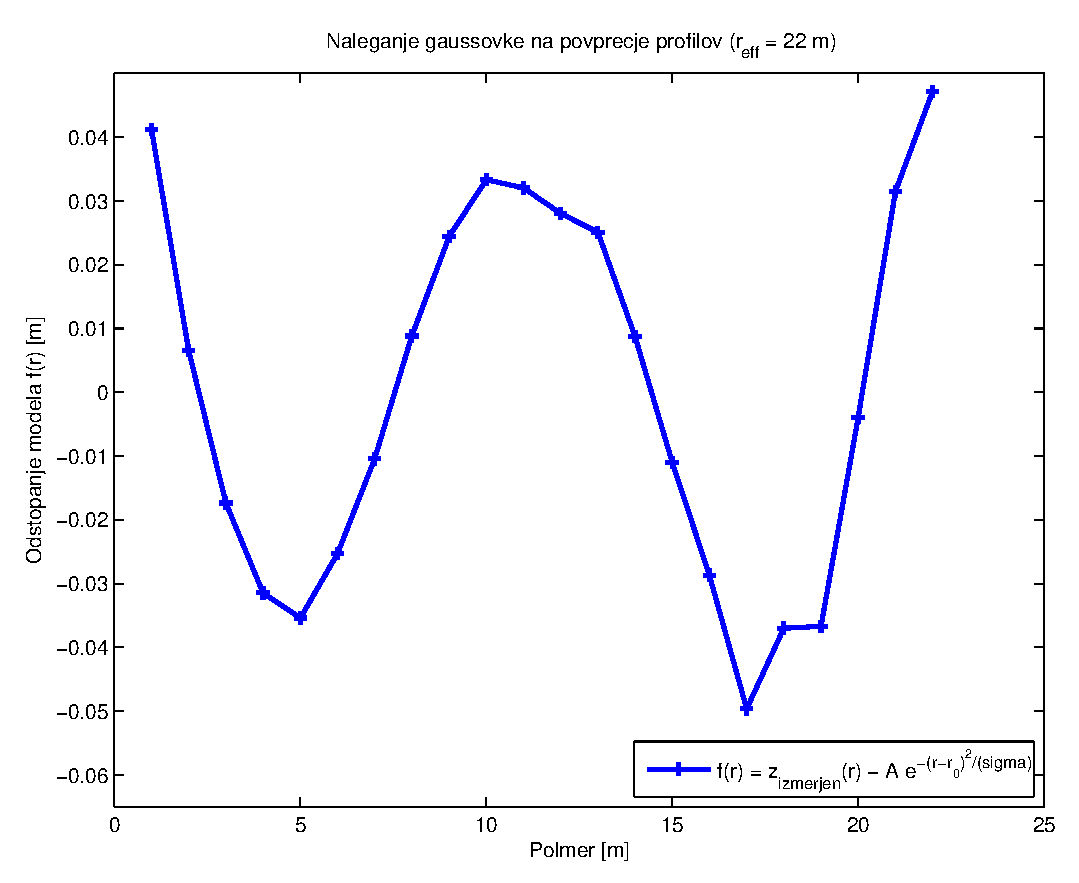
\includegraphics{slike/menisija-profil-21-fit}
          \caption{Povprecje profilov vrtač z efektivnimi polmeri med 23,5m in 24,5m. Prilegamo gaussovko (\ref{fit-profila}). Graf prikazuje razliko med povprečnim profilom in prilegano gausovko.}
          \label{fig:menisija-profil-21-fit}
        \end{figure}

        Pri tem pa je porazdelitev uteži gaussove funkcije Slika (\ref{fig:menisija-globine-hist}), porazdelitev $\sigma$ pa Slika (\ref{fig:menisija-sigme-hist}).

        \begin{figure}[H]
          \begin{center}
            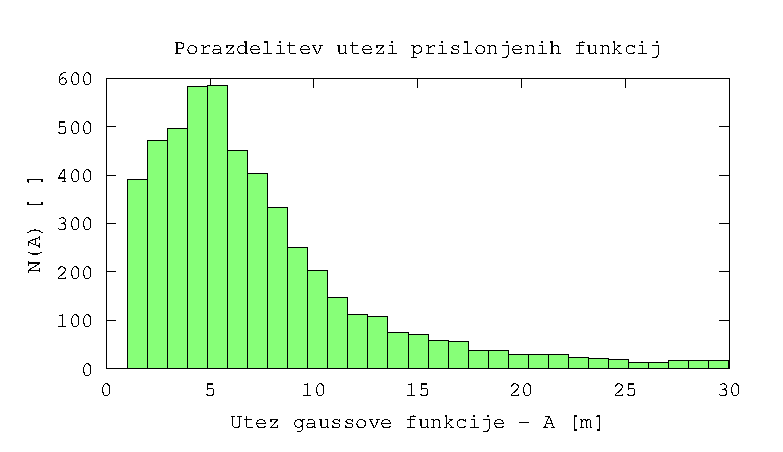
\includegraphics{slike/menisija-globine-hist}
          \end{center}
          \caption{Porazdelitev uteži A za gaussovo funkcijo prilegano na vrtače v Menišiji}
          \label{fig:menisija-globine-hist}
        \end{figure}

        \begin{figure}[H]
          \begin{center}
            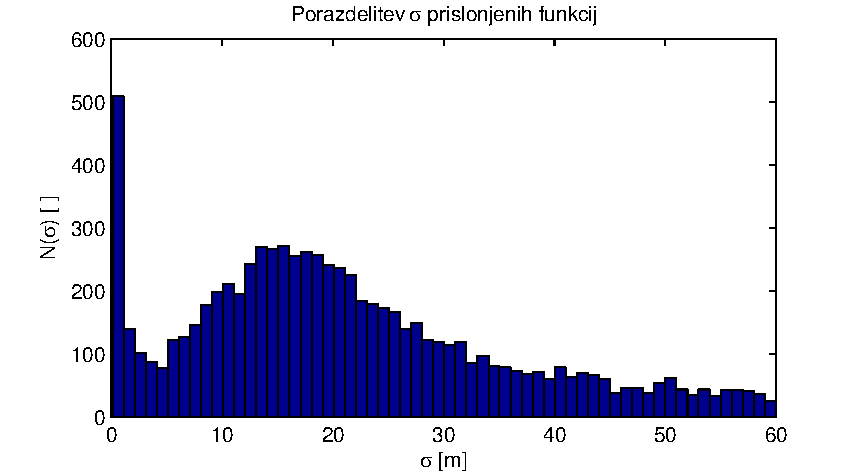
\includegraphics{slike/menisija-sigme-hist}
          \end{center}
          \caption{Porazdelitev uteži $\sigma$ za gaussovo funkcijo prilegano na vrtače v Menišiji}
          \label{fig:menisija-sigme-hist}
        \end{figure}

        Če na dobljene profile nalegamo eksponentno krivuljo (\ref{fit-profila}) in izrišemo odvisnost $\sigma_x (r_{eff})$, vidimo (Slika \ref{fig:menisija-sigma}).

        \begin{equation}
          f(r) = A \cdot e^{-\frac{(r-r_0)^2}{\sigma^2}} + C  
          \label{fit-profila}
        \end{equation}

        Odvisnost $\sigma_x(r_{eff})$ je iz naših podatkov težko določiti, zaenkrat poskusimo z linearno funkcijo (\ref{sigma-od-reff})

        \begin{equation}
          \sigma (r_{eff}) = k \cdot r_{eff} + C
          \label{sigma-od-reff}
        \end{equation}

        \begin{figure}[H]
          \centering
          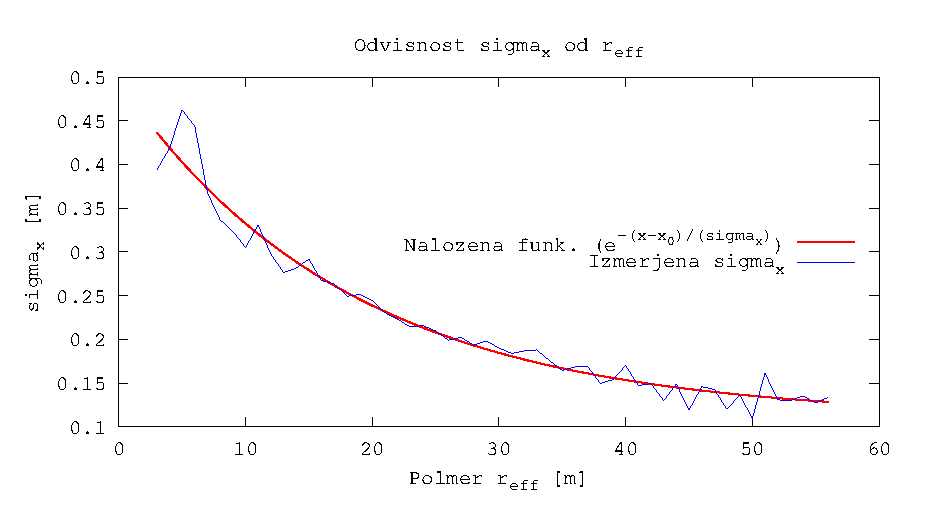
\includegraphics{slike/menisija-sigme}
          \caption{$\sigma$ s polmerom narašča}
          \label{fig:menisija-sigma}
        \end{figure}

        Na podlagi teh podatkov bi težko skleniti, da (\ref{fit-profila}) opiše profil idealne vrtače, a ujemanje je dobro in ga bomo uporabili za analitično modeliranje. 


        \chapter{Analitično modeliranje vrtač}
        \label{analiticno-modeliranje}

        \section{Model z Darcyevim tokom}

        Vzamemo, da ob deževju voda napolni porozno prst do višine $h$ in da je hitrost toka vode v prsti sorazmerna z gradientom višine - $\nabla h$. Uporabimo Darcyev zakon ($k$ je permeabilnost prsti, $g$ pa gravitacijski pospešek). (Ideja povzeta po \cite{Kodre1994})

        \begin{equation}
          \mathbf{v} = - k \rho g \nabla h
          \label{darcyev-zakon}
        \end{equation}

        Vzamemo približek, da v centru vrtače ponikne ves tok, ki priteče v vanjo:

        \begin{equation}
          \Phi_v = 2 \pi r h v
          \label{darcy-tok}
        \end{equation}

        Enačbi združimo v:

        \begin{equation}
          h \nabla h = \frac{\Phi_v}{2 \pi r v} \frac{v}{k \rho g}
          \label{darcy-pretok-1}
        \end{equation}

        Dobimo rezultat:

        \begin{equation}
          h(r_0)^2 = h(r_1)^2 - \frac{\Phi_v}{\pi k \rho g} ln(\frac{r_1}{r_0})
          \label{darcy-gladina}
        \end{equation}

        Postavimo, da je raztapljanje sorazmerno s pretokom vode:

        \begin{equation}
          \frac{\partial z}{\partial t} = C \mathbf{v} = - C k \rho g \nabla h
          \label{darcy-raztapljanje-2}
        \end{equation}

        Dobimo rezultat za z(r,t):

        \begin{equation}
          z(r,t) = z_0 - \frac{t}{2 r \sqrt{1-ln\left(\frac{1}{r}\right)}}
          \label{darcy-z}
        \end{equation}

        Rezultat seveda ni pravilen, saj neskočnih brezen na krasu ne opazimo, je pa zanimiv, kot premislek, ki pravi, da se bo še tako drobna vrtača poglabljala.

        \newpage

        \section{Difuzijski model}

        Dinamiko vrtače poskusimo opisati z nelinearno difuzijsko enačbo (\ref{nelinearna-difuzijska-enacba}). V prejšnjem poglavju smo našli nastavek za stacionano stanje (\ref{ravnovesni-nastavek-vrtace}), ki ga dopolnimo še s časovnim delom (\ref{dinamicni-nastavek-vrtace}), ter predpostavimo difuzijsko konstanto (\ref{difuzijska-konstanta-1}). Privzamemo radialno simetričnost in računamo v cilindričnih koordinatah.

        \begin{equation}
          \frac{\partial z}{\partial t} = \nabla (K(z) \nabla z)
          \label{nelinearna-difuzijska-enacba}
        \end{equation}

        \begin{equation}
          z_0(r) = z(r,\infty) = Ae^{-\left(\frac{r}{\sigma }\right)^2}
          \label{ravnovesni-nastavek-vrtace}
        \end{equation}

        \begin{equation}
          z(r,t) = A e^{-\left(\frac{r}{\sigma }\right)^2} \left(1- e^{-\frac{t}{\tau }}\right)
          \label{dinamicni-nastavek-vrtace}
        \end{equation}

        \begin{equation}
          K(z) = -\frac{\sigma ^4}{4 r^2 \tau } \left(1-\frac{A}{z_0(r)}\right) \left(1-\frac{z_0(r)}{z(r,t)}\right)
          \label{difuzijska-konstanta-1}
        \end{equation}

        Vidimo, da je tok $\mathbf{j}$:
        \begin{equation}
          \mathbf{j} = -\frac{A \sigma^2}{2 r \tau } \left( 1-e^{-(\frac{r^2}{\sigma ^2})} \right) e^{-\frac{t}{\tau }}
          \label{tok}
        \end{equation}

        Ali zapisano z $z_0(r)$ in $z(r,t)$:
        \begin{equation}
          \mathbf{j} = - K(z) \nabla z(r,t) = \frac{\sigma^2}{2 r \tau} \left(1- \frac{A}{z_0(r)}\right) (z_0(r)-z(r,t))
        \end{equation}


        Izrišemo časovno dinamiko profila vrtače (\ref{dinamicni-nastavek-vrtace}) in toka (\ref{tok}) - sliki (\ref{fig:vrtaca-dinamicno}) in (\ref{fig:tok-dinamicno}) (vzamemo $A=-6,\sigma=5,\tau = 1$).

        \begin{figure}[H]
          \begin{center}
            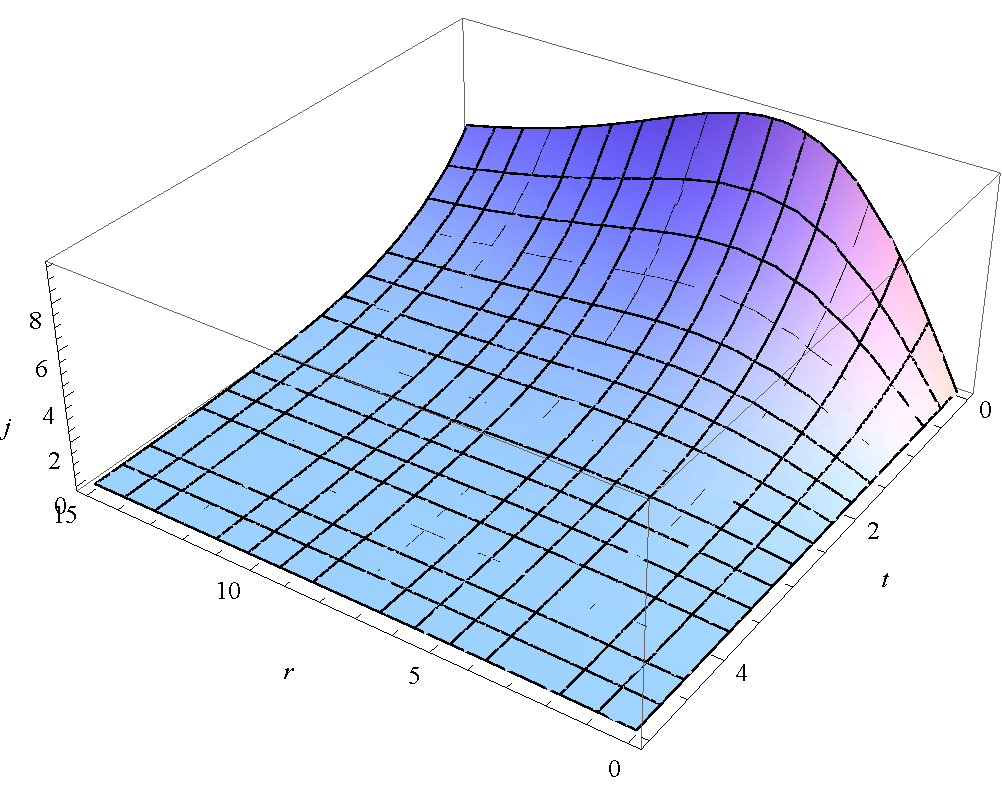
\includegraphics[width=9cm]{slike/tok-dinamicno}
          \end{center}
          \caption{Časovni razvoj toka $\mathbf{j}$, enačba (\ref{tok})}
          \label{fig:tok-dinamicno}
        \end{figure}

        \begin{figure}[H]
          \begin{center}
            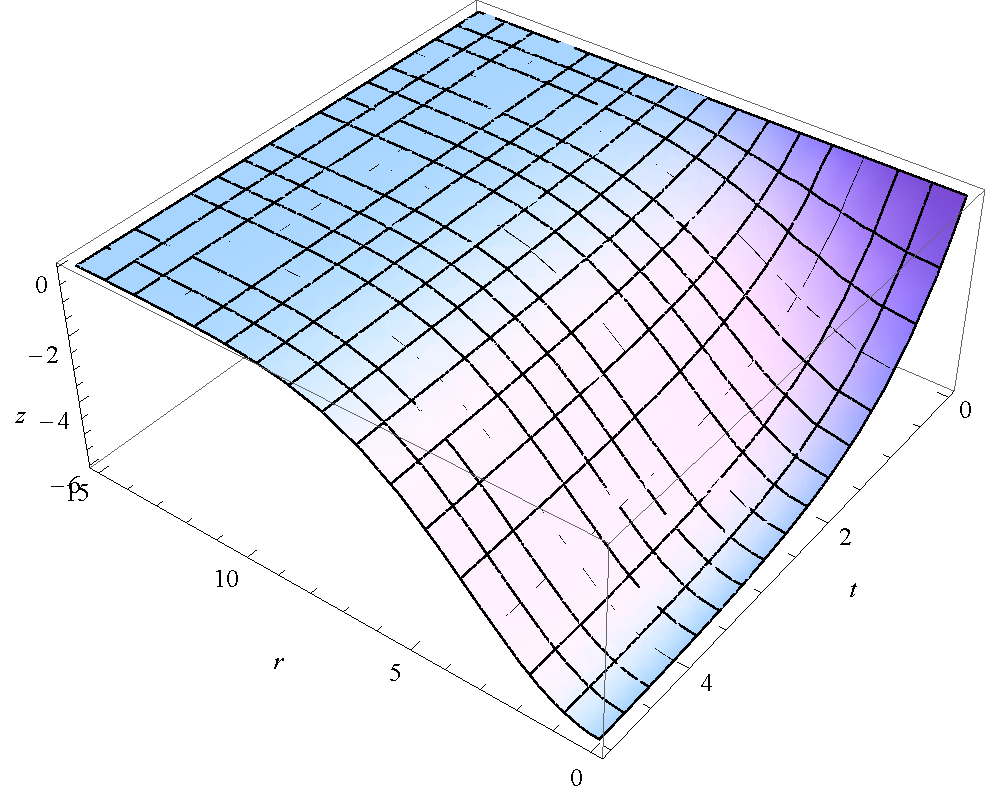
\includegraphics[width=9cm]{slike/vrtaca-dinamicno}
          \end{center}
          \caption{Časovni razvoj vrtače, po nastavku (\ref{dinamicni-nastavek-vrtace})}
          \label{fig:vrtaca-dinamicno}
        \end{figure}

\newpage

        Sedaj se postavimo daleč stran od centra vrtače, kjer po dolgem času velja:

        \begin{equation}
          \frac{\partial z}{\partial t} = -\frac{A e^{-\frac{(r \rightarrow \infty)^2}{\sigma ^2}-\frac{t \rightarrow \infty}{\tau }}}{\tau } = -\frac{A}{\tau} = v_{denudacije}
          \label{hitrost-denudacije}
        \end{equation}

        Ocenimo $\tau$ vrtač.

        \begin{equation}
          \tau = \frac{-A}{v_{denudacije}}=\frac{-5m}{-50\cdot 10^{-6} m/leto} = 10^5 leto
          \label{tau-vrtace}
        \end{equation}

        \begin{table}[H]
          \centering
          \begin{tabular}{| l | c | l | l |} \hline
            $\rho_r$ & $2700$ $kg/m^3$ & Gostota apnenca                                            \\ \hline
            $\rho_s$ & $1000$ $kg/m^3$ & Gostota delno preperele kamnine                            \\ \hline
            $C$      & $50 \cdot 10^{-6} m/leto$  & Hitrost preperevanja apnenca na ravnini         \\ \hline
            $K$      & $1 \cdot 10^{-4} m^2/leto$ & Difuzijska konstanta za delno preperelo kamnino \\ \hline
            $\sigma$ & $4.5m$ & $\sigma$ vrtače po nastavku (\ref{fit-profila})                     \\ \hline
            $A$      & $6m$ & Globina vrtače $A$ po nastavku (\ref{fit-profila})                    \\ \hline
          \end{tabular}
          \caption{Vrednosti iz literature \cite{Gams1967} \cite{ford2007karst} \cite{fleurant2008modelling} in \ref{realne-vrtace}. poglavja}
          \label{tab:tabela-konstant}
        \end{table}


        \begin{comment}

        \section{Dvofazni difuzijski model}

        Za izhodišče privzamemo difuzijski model, kot ga predlaga Heimsath \cite{Heimsath2001}.

        \begin{figure}[H]
          \centering
          \begin{tikzpicture}[
    scale=1.8,
    arrow/.style={thick,->,shorten <=-2pt, shorten >=-2pt},
    media/.style={font={\footnotesize\sffamily}}
]

    \fill[color=black!5] (0,4) coordinate (a_1) -- (6,2.5) coordinate (a_2) -- (6,0.5) coordinate (b_2) -- (0,2) coordinate (b_1)-- cycle;
    \fill[color=black!10] (b_1) -- (b_2) -- (6,0.2) coordinate (c_2) -- (0,1.7) coordinate (c_1) -- cycle;
    \fill[color=black!25] (c_1) -- (c_2) -- (6,0) -- (0,0) -- cycle;

    \path[media] (1,2.8) node [rotate=-13.5] {Delno preperela}
                            (1,2.5) node [rotate=-13.5] {kamnina, $\rho_s$}
                            (2,0.6) node [rotate=-13.5] {Nepreperela kamnina, $\rho_r$}
                            (1.3,1.5) node [rotate=-13.5] {Preperevanje};

    % Draw surface, solid rock boundary and dz_b
    \draw [thick]               (a_1) -- (a_2) node [above, xshift=-5pt] {$z$};
    \draw [thick]               (b_1) -- (b_2) node [above, xshift=-5pt] {$z_b$};
    \draw [dashed,thick] (c_1) -- (c_2);

    % Draw dr volume
    \draw (2,1.5) -- (2,3.5);
    \draw (4,1) -- (4,3);

    %Draw currents
    \draw [arrow] (1.75,2.4375) -- (2.25,2.3125) node [above=1pt] {$q_s(r)$};
    \draw [arrow] (3.75,1.9375) -- (4.25,1.8125) node [above left =9pt] {$q_s(r+dr)$};
    \draw [arrow] (2.5,1.25) -- (2.5,1.55) node [above] {$\rho_r \frac{\partial z_b}{\partial t}$};
    \draw [arrow] (3.5,1.3) -- (3.5,0.6) node [above=36] {$Q_s$};
    \draw [arrow] (3,3.1) -- (3,3.45) node [below=18pt] {$\rho_s \frac{\partial h}{\partial t}$};

    % Draw h and dz_b
    \draw [<->] (5,0.75) -- (5,2.75) node [midway, right] {$h$};
    \draw [<->] (5,0.45) -- (5,0.75) node [midway, right, yshift=-0pt,rotate=-13.5] {$dz_b$};

    % Draw axes
    \draw [<->,thick] (0,4.3) node (yaxis) [above] {$z$}
        |- (6.3,0) node (xaxis) [right] {$r$};

\end{tikzpicture}
          \caption{Skica difuzijskega modela nastajanja vrtače}
          \label{fig:difuzijski-model}
        \end{figure}

        \begin{equation}
          \rho_s \frac{\partial h}{\partial t} = -\rho_r \frac{\partial z_b}{\partial t} - \nabla q_s
          \label{kontinuitetna-enacba-original}
        \end{equation}

        Kjer je $h$ višina stolpca sedimenta, $z_b$ višina skalne podlage, $z$ višina površja, $\rho_r$ in $\rho_s$ gostoti skalne podlage in sedimenta, $q_s$ pa gostota toka sedimenta. Za gostoto toka sedimenta vzamemo, da je sorazmeren z naklonom površja:
        \begin{equation}
          q_s = - \rho_s K \nabla z
          \label{difuzijski-tok}
        \end{equation}

        Kjer je $K$ analogna konstanta difuzijski.
        Model dopolnimo z raztapljanjem in izpiranjem delno raztopljene kamnine v podzemlje - to pospravimo v člen $Q_s$ in vstavimo \ref{difuzijski-tok}.
        \begin{equation}
          \rho_s \frac{\partial h}{\partial t} = -\rho_r \frac{\partial z_b}{\partial t} + K \rho_s \Delta z - Q_s
          \label{kontinuitetna-enacba-1}
        \end{equation}

        Dobljen model skiciramo na Sliko \ref{fig:difuzijski-model}.

        V ravnovesnem stanju vrtače, ki smo ga domnevno našli v \ref{realne-vrtace}. poglavju (enačba \ref{fit-profila}) zahtevamo, da velja $\frac{\partial h}{\partial t} = 0$ in $\frac{\partial z_b}{\partial t} = C$, kjer $C<0$, saj se meja preperelosti znižuje. Dobimo:

        \begin{equation}
          Q_s = - \rho_r C + \rho_s K \Delta z
          \label{kontinuitetna-enacba-ravnovesje}
        \end{equation}

        Vstavimo ravnovesni profil vrtače (enačba \ref{fit-profila}) in vrednosti iz tabele (\ref{tab:tabela-konstant}), da dobimo profil $Q_s$ profil raztapljanja apnenca v na površju (Slika (\ref{fig:profil-raztapljanja})).


        \begin{figure}[H]
          \begin{center}
            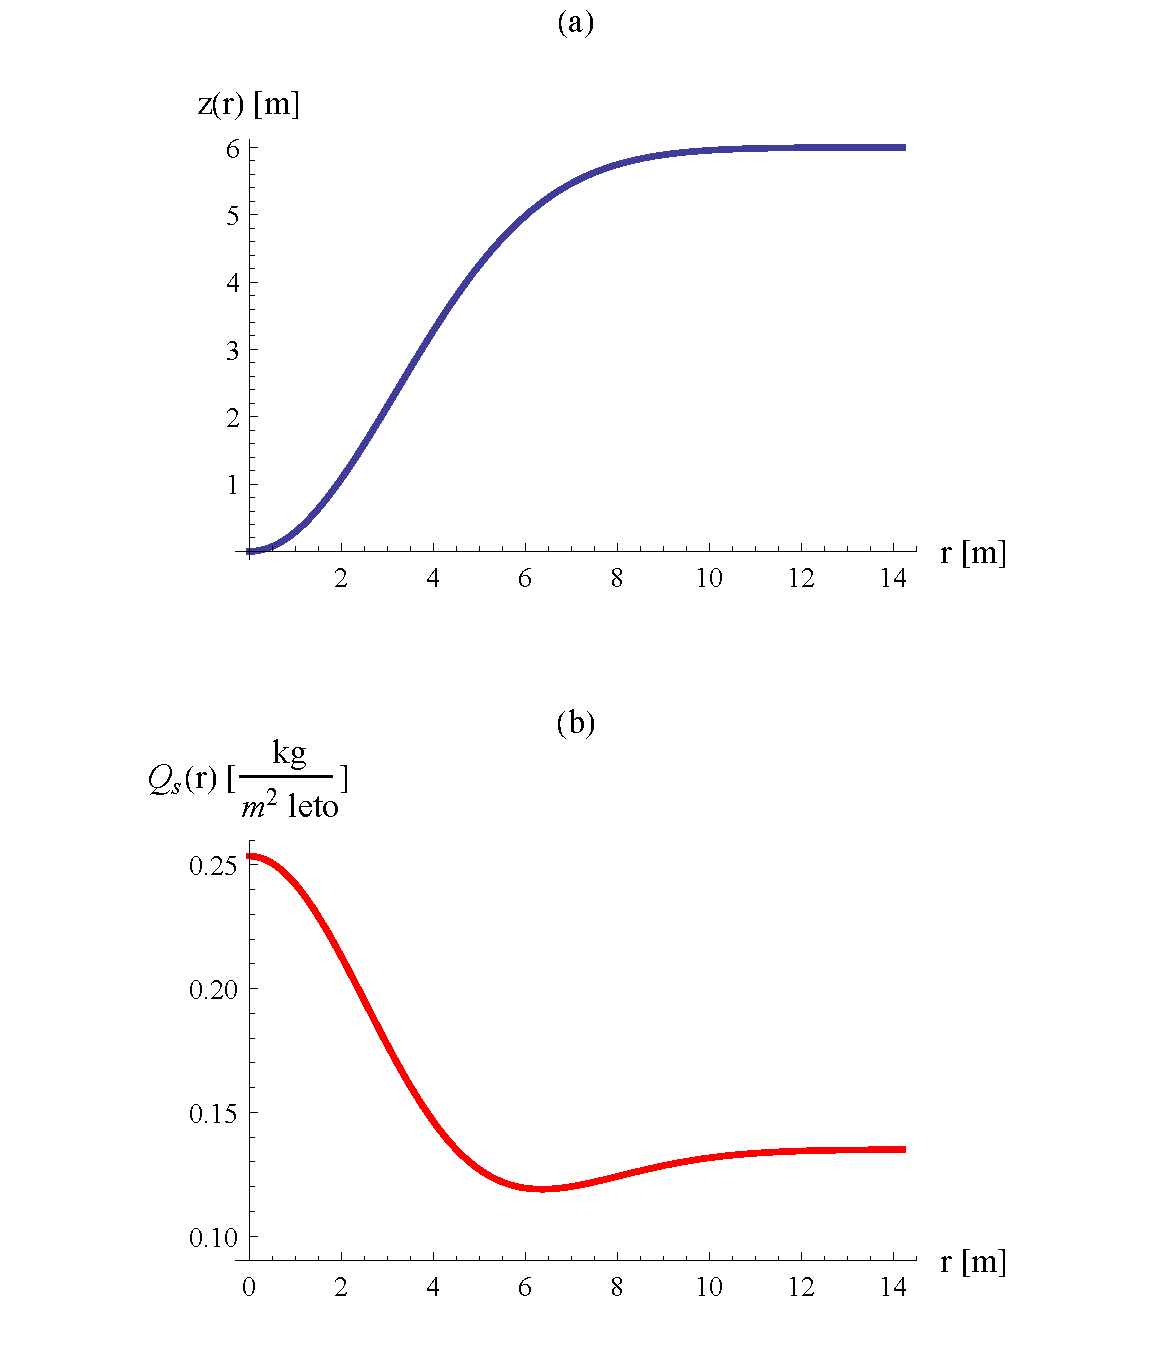
\includegraphics[width=10cm]{slike/profil-raztapljanja}
          \end{center}
          \caption{(a) Profil vrtače (b) modeliran profil raztapljanja delno preperele kamnine}
          \label{fig:profil-raztapljanja}
        \end{figure}

        Dobljeni profil raztapljanja nakazuje kvalitativno podobnost meritvam, ki jih je opravil Zambo (\cite{Zambo1997}) v osemdesetih (Slika \ref{fig:vrtaca-aggtelek}).

        \begin{figure}[H]
          \begin{center}
            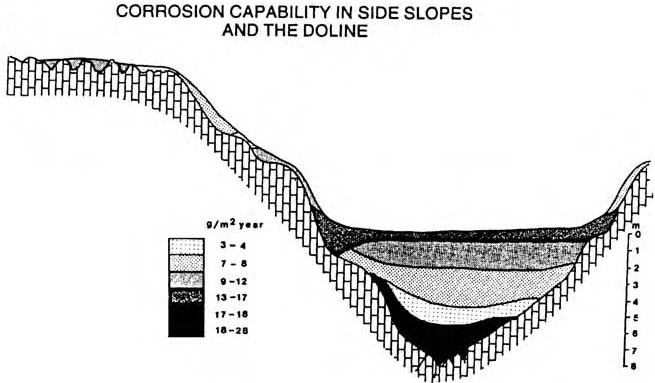
\includegraphics[width=10cm]{slike/vrtaca-aggtelek}
          \end{center}
          \caption{Meritve raztapljanja apnenca v realni vrtači - dolina Beke, nacionalni park Aggtelek na Madžarskem \cite{Zambo1997}}
          \label{fig:vrtaca-aggtelek}
        \end{figure}

        Profil vrtače blizu ravnovesja zmotimo s spremembo vrednosti oblike profila ($z(r)$), vstavimo nastavek za $\frac{\partial z_b}{\partial t}=\frac{1}{|h_0-h|}$ in \dots


        \section{Elastomehanični model}
        \section{Boussinesqov približek}

        \chapter{Numerično modeliranje vrtač} 
        \section{Model naključnih korozijskih točk}
        \section{Naključne korozijske točke na realni kamnini}
        \section{Preizkus modela korozijskih točk na geološki karti}

        \end{comment}

        \section{Kardar-Parisi-Zhang}
        Za opis področja vrtač uporabimo analogijo z rastjo vmesnikov - npr. nabiranjem vodnega kamna - le da tu nebo raste v apnenčasto podlago.
        Za izhodišče vzamemo stohastično diferencialno Kardar-Parisi-Zhang enačbo (\cite{kardar1986dynamic}):

        \begin{equation}
          \frac{\partial h}{\partial t} = \nu \nabla^2 h + \frac{\lambda}{2} (\nabla h)^2 + \eta (\mathbf{x},t)
          \label{KPZ}
        \end{equation}

        $\eta(\mathbf{x},t)$ je bel Gaussov šum, za katerega velja $\eta(\mathbf{x},t)$ 


        \chapter{Zaključek}

        Izkaže se, da je zaznava in segmentacija vrtač na digitalnem modelu reliefu relativno enostavna naloga, izvedljiva na osebnem računalniku. Kodo, ki sem jo za ta postopek spisal, sem dokumentirano objavil na spletu in bo morda še služila za obsežnejšo katalogizacijo vrtač.
        Za nekoliko težjo nalogo se izkaže določanje idealne oblike vrtače, saj le-ta ne obstaja, in bi se moralo pravo vprašanje glasiti, kakšna je idealna oblika vrtače na izotropni podlagi po dolgem času. Vseeno sem se odločil, da za idealno vrtačo vzamem povprečje velike količine vrtač.

        Precej zahtevnejša naloga je bila izbira fizikalnega modela in dinamičnega opisa vrtače. Najbolj primeren model se je zdela nelinearna difuzijska enačba s primerno izbrano difuzijsko konstanto, ki je omogočila rešitev z previdno izbranim dinamičnim nastavkom. Treba je priznati, da je taka rešitev krhka in verjetno vsaj delno napačna, a nam nakaže možnost, da je originalna teza o tem da so vrtače ravnovesne reštive lahko pravilna.
        Za popolnejši študij in dober model vrtač bi verjetno potrebovali bolj poglobljene informacije o prsti, geoloških in bioloških dejavnikih, ki lahko vplivajo na časovno dinamiko terena. Zanimiva ideja bi bila z geološkim študijem najti vrtače v različnih stopnjah razvoja in s pomočjo te informacije oblikovati dinamičen nastavek, na podlagi katerega bi potem morda bolj osvetlili dinamično enačbo.

        \nocite{*}
        \newpage
        \bibliography{bibliography}{}
        \bibliographystyle{alpha}


        \end{document}

